\documentclass{aitemplate}

\usepackage{textcomp}
\usepackage{ai}
\usepackage{alltt}
\usepackage{tikz}
\usepackage{listings}

\begin{document}

\printtitle{1}

\section*{Ejercicio 1}
\begin{aibox}{\function}
;; h-mapcar

SYNTAX: h-mapcar (x w sigma) 
\end{aibox}

\begin{aibox}{\examples}
\begin{alltt}
\end{alltt}

\end{aibox}

\begin{aibox}{\comments}

\end{aibox}
\begin{aibox}{\answers}

\end{aibox}
\begin{aibox}{\othercomments}

\end{aibox}
\begin{aibox}{\pseudocode}

\end{aibox}
\begin{aibox}{\code}

\begin{alltt}
;;%% code

(defun h-mapcar (x w sigma) 
    (funcall sigma 
        (reduce #'+
            (mapcar #'* x w))))

\end{alltt}
\end{aibox}

%\newpage
%\begin{aibox}{\function}
;; h-recursive-aux

SYNTAX: h-recursive-aux (x w acc)
\end{aibox}

\begin{aibox}{\examples}
\begin{alltt}
\end{alltt}

\end{aibox}

\begin{aibox}{\comments}

\end{aibox}
\begin{aibox}{\answers}

\end{aibox}
\begin{aibox}{\othercomments}

\end{aibox}
\begin{aibox}{\pseudocode}

\end{aibox}
\begin{aibox}{\code}

\begin{alltt}
;;%% code

(defun h-recursive-aux (x w acc)
        (if (null x)
            acc
        (h-recursive-aux (rest x) (rest w) ( + (* (first x)  (first w)) acc))))
\end{alltt}
\end{aibox}

\newpage
\begin{aibox}{\function}
;; h-recursive

SYNTAX: h-recursive (x w sigma) 
\end{aibox}

\begin{aibox}{\examples}
\begin{alltt}
(H-RECURSIVE '(0.1 -0.5 0.7) '(-0.1 0.2 0.3) #'logit); 0.4750208
(H-RECURSIVE '(0.1 -0.5 0.7) '(-0.1 0.2 0.3) #'TANHIP); 0.09966801

(H-RECURSIVE '(0.1 -0.5 0.7) '(-0.1 1) #'TANHIP); ERROR
(H-RECURSIVE '(0.1 -0.5 0.7) '() #'tanhip) ERROR
\end{alltt}
\end{aibox}

\begin{aibox}{\comments}
Salen los mismos resultados que con la función H-MAPCAR, como podíamos esperar. 

Simplemente hay que tener cuidado con que las listas deben tener la misma longitud para que funcione correctamente.
\end{aibox}
\begin{aibox}{\answers}
No hay preguntas en el enunciado.
\end{aibox}
\begin{aibox}{\othercomments}
Utilizamos la llamada a la función auxiliar para optimizar el uso de la recursión. Con el uso de un acumulador conseguimos evitar la cadena de devoluciones para resolver la recursión.

Incluimos el código de la función auxiliar empleada en el apartado de código.
\end{aibox}

\begin{aibox}{\pseudocode}
Esta es la versión inicial en la que pensamos que no incluía el acumulador: 
\begin{alltt}
h-recursiva (x w sigma)
     (sigma(first(x)*first(w)) + h-recursive(rest(x),rest(w),sigma))
\end{alltt}
\end{aibox}
\begin{aibox}{\code}

\begin{alltt}

(defun h-recursive (x w sigma) 
        (funcall sigma (h-recursive-aux x w 0)))

(defun h-recursive-aux (x w acc)
    (if (null x)
          acc
    (h-recursive-aux (rest x) (rest w) ( + (* (first x)  (first w)) acc))))


\end{alltt}
\end{aibox}

%\newpage
%\input{Memoria/ej1.lisplogit.tex}
%\newpage
%\input{Memoria/ej1.lisptanhip.tex}
%\newpage
%\begin{aibox}{\function}
;; combine-elt-lst-app

SYNTAX: combine-elt-lst-app (elt lst)
\end{aibox}

\begin{aibox}{\examples}
\begin{alltt}
\end{alltt}

\end{aibox}

\begin{aibox}{\comments}

\end{aibox}
\begin{aibox}{\answers}

\end{aibox}
\begin{aibox}{\othercomments}

\end{aibox}
\begin{aibox}{\pseudocode}

\end{aibox}
\begin{aibox}{\code}

\begin{alltt}
;;%% code

(defun combine-elt-lst-app (elt lst)
            (mapcar #'(lambda (x) (append (list elt) x)) lst))

\end{alltt}
\end{aibox}

\newpage

\section*{Ejercicio 2}

\begin{aibox}{\function}
;; combine-elt-lst

SYNTAX: combine-elt-lst (elt lst)
\end{aibox}

\begin{aibox}{\examples}

\begin{alltt}
(combine-elt-lst 'a '(1 2 3)); ((A 1) (A 2) (A 3))

(combine-elt-lst 'a '()); NIL
\end{alltt}

\end{aibox}

\begin{aibox}{\comments}
\end{aibox}
\begin{aibox}{\answers}

\end{aibox}
\begin{aibox}{\othercomments}

\end{aibox}
\begin{aibox}{\pseudocode}

\end{aibox}
\begin{aibox}{\code}

\begin{alltt}

(defun combine-elt-lst (elt lst)
            (mapcar #'(lambda (x) (list elt x)) lst))

\end{alltt}
\end{aibox}

%\newpage
%\begin{aibox}{\function}
;; combine-lst-lst-app

SYNTAX: combine-lst-lst-app (lst1 lst2)
\end{aibox}

\begin{aibox}{\examples}
\begin{alltt}
\end{alltt}

\end{aibox}

\begin{aibox}{\comments}

\end{aibox}
\begin{aibox}{\answers}

\end{aibox}
\begin{aibox}{\othercomments}

\end{aibox}
\begin{aibox}{\pseudocode}

\end{aibox}
\begin{aibox}{\code}

\begin{alltt}
;;%% code

(defun combine-lst-lst-app (lst1 lst2)
            (mapcan #'(lambda (x) (combine-elt-lst-app x lst2)) lst1))

\end{alltt}
\end{aibox}

\newpage
\begin{aibox}{\function}
\begin{alltt}
;; combine-lst-lst

SYNTAX: combine-lst-lst (lst1 lst2)
RECIBE: Dos listas.
EVALÚA A: Una lista de todas las posibles combinaciones de un elemento de lst1 con un 
elemento de lst2, también conocido como producto cartesiano.
\end{alltt}
\end{aibox}

\begin{aibox}{\examples}
\begin{alltt}
(combine-lst-lst '(a b c) '(1 2))
; ((A 1) (A 2) (B 1) (B 2) (C 1) (C 2))

(combine-lst-lst '(a b c) '()); NIL

(combine-lst-lst '() '(a b c)); NIL
\end{alltt}

\end{aibox}

\begin{aibox}{\comments}

\paragraph{}
Utilizamos la función definida en el ejercicio anterior (combine-elt-lst) lo que facilita la tarea.
\paragraph{}
En este ejercicio vimos la diferencia entre mapcan y mapcar. Necesitábamos que el resultado fuera 1 única lista con todos los elementos y no una lista de listas. Este conocimiento fue realmente útil en la resolución del siguiente ejercicio.
\end{aibox}
\begin{aibox}{\pseudocode}
Esta primera aproximación (traducida a programación funcional utilizando \emph{mapcar}) luego fue modificada (por el uso de mapcan en vez de mapcar) para que el resultado fuera una única lista de átomos.
\begin{alltt}
combine-lst-lst (lst1,lst2)
    Para cada eltemento en lst1:
        combine-elt-lst (elemento,lst2)
\end{alltt}
\end{aibox}
\begin{aibox}{\code}

\begin{alltt}

(defun combine-lst-lst (lst1 lst2)
            (mapcan #'(lambda (x) (combine-elt-lst x lst2)) lst1))

\end{alltt}
\end{aibox}

\newpage
\begin{aibox}{\function}
;; combine-lst-of-lst

SYNTAX: combine-lst-of-lst (lst)
\end{aibox}

\begin{aibox}{\examples}
\begin{alltt}
 (combine-lst-of-lst '((a b c) (+ -) (1 2 3)))

;((A + 1) (A + 2) (A + 3) (A - 1) (A - 2) (A - 3) (B + 1) (B + 2) (B + 3)
; (B - 1) (B - 2) (B - 3) (C + 1) (C + 2) (C + 3) (C - 1) (C - 2) (C - 3))

(combine-lst-of-lst '((a b) (+ -) (1 2) (NIL T)))

; ((A + 1 NIL) (A + 1 T) (A + 2 NIL) (A + 2 T) (A - 1 NIL) (A - 1 T) (A - 2 NIL)
; (A - 2 T) (B + 1 NIL) (B + 1 T) (B + 2 NIL) (B + 2 T) (B - 1 NIL) (B - 1 T)
; (B - 2 NIL) (B - 2 T))

(combine-lst-of-lst '((a b) (+ -) (1 2) ()))
; NIL
\end{alltt}

\end{aibox}

\begin{aibox}{\comments}
Esta función utiliza una combinación de elemento con lista distinta. 

La hemos definido de forma recursiva (que nos parecía más fácil de pensar) pero utilizando una combinación de elemento con lista distinta a la del ejercicio 1, pero sólo en el caso recursivo. En el caso base hemos mantenido la función del ejercicio 2.1. 

Esta decisión la tomamos para obtener como resultado una única lista de listas, con únicamente 2 niveles y no más. Empleando la función del ejercicio 2.1 no funcionaba correctamente este requisito.

\end{aibox}
\begin{aibox}{\answers}

\end{aibox}
\begin{aibox}{\othercomments}

Las funciones auxiliares definidas son combine-lst-lst-app que simplemente llama a la función combine-elt-lst-app que utiliza \emph{cons} en vez de \emph{list}.

Hemos pensado que no hacía falta rellenar la ficha de las funciones auxiliares (debido a su gran similitud con las soluciones de los ejercicios 2.1 y 2.2).

\end{aibox}
\begin{aibox}{\pseudocode}
funcion CombinarListaDeListas:
	Si (la lista tiene 2 listas)
		CombinarListas(sublista1,sublista2)
	sino
		CombinarListas (Primera\_Sublista, CombinarListaDeListas (RestoDeSublistas))

\end{aibox}
\begin{aibox}{\code}

\begin{alltt}
(defun combine-lst-of-lst (lst)
    (if (null (cddr lst))
            (combine-lst-lst (car lst) (cadr lst))
    (combine-lst-lst-app (car lst) (combine-lst-of-lst (cdr lst)))))

\end{alltt}
\end{aibox}

\newpage

\section*{Ejercicio 3}
\begin{aibox}{\function}
\begin{alltt}
;; eval-fbf

SYNTAX: eval-fbf (fbf int)
RECIBE: fórmula bien formada e interpretación
EVALÚA A : Valor de verdad de la fbf con la interpretación dada

\end{alltt}
\end{aibox}

\begin{aibox}{\examples}
\begin{alltt}
(eval-fbf '(<=> T NIL) '())
; NIL
(eval-fbf '(=> A NIL) '((A T)))
; NIL
(eval-fbf '(<=> P (^ A  H)) '((A NIL) (P NIL) (H T)))
; T
(eval-fbf '(<=> (v A P H) (^ A P H)) '((A NIL) (P NIL) (H T)))
; NIL
\end{alltt}

\end{aibox}

\begin{aibox}{\comments}
La función \texttt{evaluator} devuelve la función correspondiente al operador pasado como argumento. Después de evaluar todos los elementos de la lista de forma recursiva con \texttt{eval-fbf}, aplicamos el evaluador con los elementos de la lista como argumentos.
\end{aibox}

\begin{aibox}{\pseudocode}
\begin{alltt}
si fbf es un átomo
	obtener valor de verdad de fbf con interp.
si no
	sym = primer elemento de fbf
	evaluator = obtener función evaluadora para el operador
	results = eval-fbf(resto de elementos de la fbf)
	llamar a evaluator con results como argumentos

\end{alltt}
\end{aibox}
\begin{aibox}{\code}

\begin{alltt}
(defun eval-fbf (fbf int)
   	(if (atom fbf)
         (getint fbf int)
         (apply 
           (evaluator (first fbf)) 
           (mapcar #'(lambda (f) (eval-fbf f int)) (rest fbf)))))

\end{alltt}
\end{aibox}

\newpage
\begin{aibox}{\function}
;; encuentra-modelos

SYNTAX: encuentra-modelos (kb) 
\end{aibox}

\begin{aibox}{\examples}
\begin{alltt}
(encuentra-modelos '((=> A (¬ H)) (<=> P (^ A  H)) (=> H P))) ;
 (((A T) (P NIL) (H NIL)) ((A NIL) (P NIL) (H NIL)))

(encuentra-modelos '((=> (^ P I)  L)  (=> (¬ P) (¬ L)) (¬ P) L)) ;
 NIL

\end{alltt}

\end{aibox}

\begin{aibox}{\comments}

\end{aibox}
\begin{aibox}{\answers}

\end{aibox}
\begin{aibox}{\othercomments}

\end{aibox}
\begin{aibox}{\pseudocode}

\end{aibox}
\begin{aibox}{\code}

\begin{alltt}

(defun encuentra-modelos (kb) 
  (remove-if-not 
    #'(lambda (int) (interpretacion-modelo-p kb int)) 
    (genera-lista-interpretaciones (extrae-simbolos kb))))

\end{alltt}
\end{aibox}

\newpage
\begin{aibox}{\function}
\begin{alltt}
;; extrae-simbolos

SYNTAX: extrae-simbolos (expr)
RECIBE : fórmula bien formada en cualquier formato (expr)
EVAlÚA A: Lista de símbolos atómicos (sin repeticiones)
	utilizados en la fórmula bien formada. El orden en la lista no es
	relevante.

\end{alltt}
\end{aibox}

\begin{aibox}{\examples}
\begin{alltt}
(extrae-simbolos '((=> (^ P I) L) (=> (¬ P) (¬ L)) (¬ P) (L)))
;; (I P L)
(extrae-simbolos '((<=> (¬ (P ^ L)) (v (¬ (=> K P)) K P))))
;; (L K P)
\end{alltt}

\end{aibox}

\begin{aibox}{\comments}
Para extraer los símbolos, aplanamos la lista (nos quitamos los paréntesis anidados), eliminamos todo lo que no sea un símbolo (\texttt{symbol-p} devuelve T si el argumento no es ni un conector ni \texttt{T} o \texttt{nil}) y eliminamos posibles duplicados.
\end{aibox}

\begin{aibox}{\pseudocode}
\begin{alltt}
symbols = ()

for atom in (flatten expr):
    if (symbol-p atom)
        append atom to symbols

remove duplicates in symbols
return symbols

\end{alltt}
\end{aibox}

\begin{aibox}{\code}

\begin{alltt}

(defun extrae-simbolos (expr)
    (remove-duplicates (remove-if-not #'symbol-p (flatten expr))))

\end{alltt}
\end{aibox}

\newpage
\begin{aibox}{\function}
\begin{alltt}
;; genera-lista-interpretaciones

SYNTAX: genera-lista-interpretaciones (lst) 
RECIBE   : Lista de N símbolos atómicos
EVALÚA A : Lista de 2^N posibles interpretaciones
             (lista de pares (<símbolo> <valor de verdad>))

\end{alltt}
\end{aibox}

\begin{aibox}{\examples}
\begin{alltt}
(genera-lista-interpretaciones '(P I L))
;;; (((P T) (I T) (L T)) ((P T) (I T) (L NIL)) ((P T) (I NIL) (L T))
 ((P T) (I NIL) (L NIL)) ((P NIL) (I T) (L T)) ((P NIL) (I T) (L NIL))
 ((P NIL) (I NIL) (L T)) ((P NIL) (I NIL) (L NIL)))
 (genera-lista-interpretaciones '(A))
;;; (((A T) (A NIL)))
\end{alltt}

\end{aibox}

\begin{aibox}{\comments}
Primero generamos todas las posibles interpretaciones de cada átomo (que solo puede ser T y NIL) y formamos una lista de listas de la forma (((Atomo1 T) (Atomo1 NIL)) ((Atomo2 T)(Atomo2 NIL)) ...)

Ahora solo falta combinar estas listas (con la función del ejericico 2.3) para conseguir todas las posibles combinaciones.

Al realizar este ejercicio nos dimos cuenta de un error en la función combine-lst-of-lst que tuvimos que corregir.
\end{aibox}

\begin{aibox}{\pseudocode}
\begin{alltt}
genera-lista-interpretaciones (lst)
    para cada elemento en lst
        añadir ( combinar(elemento, (T, NIL), aux)
    combine-lst-of-lst (aux)
\end{alltt}
\end{aibox}
\begin{aibox}{\code}

\begin{alltt}
(defun genera-lista-interpretaciones (lst) 
    (combine-lst-of-lst (mapcar #'(lambda (x) (combine-elt-lst x '(T NIL))) lst)))
\end{alltt}
\end{aibox}

\newpage
\begin{aibox}{\function}
\begin{alltt}
;; interpretacion-modelo-p

SYNTAX: interpretacion-modelo-p (kb interpretacion) 
RECIBE: - kb. Lista de fbfs.
		- interpretacion. Lista con asignaciones de valores de verdad a cada símbolo.

\end{alltt}
\end{aibox}

\begin{aibox}{\examples}
\begin{alltt}
(interpretacion-modelo-p 
 '((<=> A (¬ H)) (<=> P (^ A  H)) (<=> H P)) '((A NIL) (P NIL) (H T)))
 ;;; NIL

(interpretacion-modelo-p
 '((<=> A (¬ H)) (<=> P (^ A  H)) (<=> H P)) '((A T) (P NIL) (H NIL)))
;;; T
\end{alltt}
\end{aibox}

\begin{aibox}{\comments}
Evaluamos todas las fbf de la base de conocimiento y nos aseguramos que todas sean \texttt{T} con \texttt{every identity}.
\end{aibox}

\begin{aibox}{\pseudocode}
\begin{alltt}
evaluations = eval-fbf for each fbf in kb
return every evaluation in evaluations is T

\end{alltt}
\end{aibox}
\begin{aibox}{\code}

\begin{alltt}

(defun interpretacion-modelo-p (kb interpretacion) 
  (every #'identity (mapcar #'(lambda (fbf) (eval-fbf fbf interpretacion)) kb)))

\end{alltt}
\end{aibox}

\newpage
\begin{aibox}{\function}
\begin{alltt}
;; SAT-p

SYNTAX: SAT-p (kb)
RECIBE   : base de conocimiento (KB)
EVALÚA A : T si existe al menos un modelo para kb
            NIL en caso contrario
\end{alltt}
\end{aibox}

\begin{aibox}{\examples}
\begin{alltt}
(SAT-p '((<=> A (¬ H)) (<=> P (^ A H)) (<=> H P))) 
; T

(SAT-p '((=> (^ P I) L) (=> (¬ P) (¬ L)) (¬ P) L)) 
; NIL
\end{alltt}

\end{aibox}

\begin{aibox}{\comments}
Esta función simplemente verifica que la lista de modelos de la base de conocimiento no sea vacía.
\end{aibox}
\begin{aibox}{\pseudocode}
\begin{alltt}
mods = encontrar modelos de kb
si mods es vacía
    devolver NIL
si no
    devolver T
\end{alltt}
\end{aibox}
\begin{aibox}{\code}

\begin{alltt}

(defun SAT-p (kb)
  (not (null (encuentra-modelos kb))))

\end{alltt}
\end{aibox}

\newpage
%\input{Memoria/ej3.lisptruth-value-p.tex}
%\newpage

\section*{Ejercicio 4}

\paragraph*{I)} El algoritmo de búsqueda en anchura expande un nodo, y después explora todos sus hijos. La implementación se haría con una cola FIFO: exploramos un nodo y añadimos sus hijos a la cola de abiertos, de tal forma que el orden de exploración va de forma descendiente, de nodos más cercanos a la raíz a los más alejados.

\begin{figure}[hbtp]
\centering
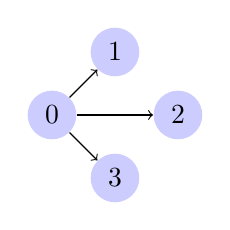
\begin{tikzpicture}[scale=.8,auto=left,every node/.style={circle,fill=blue!20}]
\node (A) at (0,0) {0};
\node (B) at (2,0) {2};
\node (C) at (1,1) {1};
\node (D) at (1,-1) {3};

\draw[->] (A) -- (B);
\draw[->] (A) -- (C);
\draw[->] (A) -- (D);
\end{tikzpicture}
\caption{Caso típico (I) de búsqueda en anchura}
\end{figure}

\begin{figure}[hbtp]
\centering
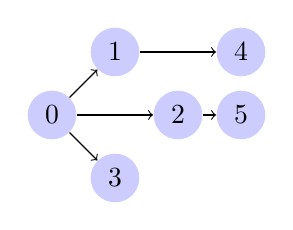
\begin{tikzpicture}[scale=.8,auto=left,every node/.style={circle,fill=blue!20}]
\node (A) at (0,0) {0};
\node (B) at (2,0) {2};
\node (C) at (1,1) {1};
\node (D) at (1,-1) {3};
\node (E) at (3,0) {5};
\node (F) at (3,1) {4};

\draw[->] (A) -- (B);
\draw[->] (A) -- (C);
\draw[->] (A) -- (D);
\draw[->] (C) -- (F);
\draw[->] (B) -- (E);
\end{tikzpicture}
\caption{Caso típico (II) de búsqueda en anchura}
\end{figure}


\begin{figure}[hbtp]
\centering
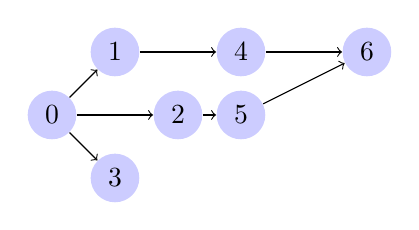
\begin{tikzpicture}[scale=.8,auto=left,every node/.style={circle,fill=blue!20}]
\node (A) at (0,0) {0};
\node (B) at (2,0) {2};
\node (C) at (1,1) {1};
\node (D) at (1,-1) {3};
\node (E) at (3,0) {5};
\node (F) at (3,1) {4};
\node (G) at (5,1) {6};

\draw[->] (A) -- (B);
\draw[->] (A) -- (C);
\draw[->] (A) -- (D);
\draw[->] (C) -- (F);
\draw[->] (B) -- (E);
\draw[->] (F) -- (G);
\draw[->] (E) -- (G);
\end{tikzpicture}
\caption{Caso especial: grafo no árbol}
\end{figure}

\begin{figure}[hbtp]
\centering
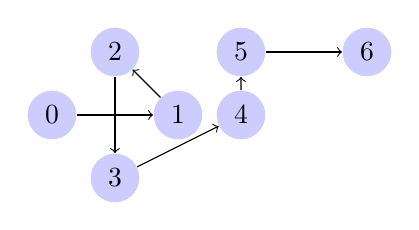
\begin{tikzpicture}[scale=.8,auto=left,every node/.style={circle,fill=blue!20}]
\node (A) at (0,0) {0};
\node (B) at (2,0) {1};
\node (C) at (1,1) {2};
\node (D) at (1,-1) {3};
\node (E) at (3,0) {4};
\node (F) at (3,1) {5};
\node (G) at (5,1) {6};

\draw[->] (A) -- (B);
\draw[->] (B) -- (C);
\draw[->] (C) -- (D);
\draw[->] (D) -- (E);
\draw[->] (E) -- (F);
\draw[->] (F) -- (G);
\end{tikzpicture}
\caption{Caso especial: grafo estilo lista}
\end{figure}

\paragraph{II)} Ese código explora todo el grafo, y está claro que si los dos nodos están conectados, encontrará un camino. La cuestión está en discernir si hay un camino más corto que el que encuentra la función.

Para nuestros propósitos, podemos reescribir el grafo de búsqueda como un árbol en el que la raíz es el nodo origen de la búsqueda y los nodos a nivel $n$ son los nodos que están a distancia $n$ del origen. A efectos de la búsqueda en anchura para buscar un camino, es equivalente buscar en el grafo original que en este árbol. Entonces, si encontramos el nodo destino en el nivel $k$ es imposible que haya un camino más corto, ya que el algoritmo explora por completo cada nivel antes de pasar al siguiente y habría encontrado el camino más corto antes.

\paragraph{III)}
\begin{lstlisting}
funcion bfs(destino, cola, grafo)
	si cola == nil:
		devolver nil
	
	cola[0] -> path
	path[0] -> node
	
	si el nodo es el destino:
		invertir path
		devolver path
	si no
		llamar a bfs
	
\end{lstlisting}

\end{document}
